\documentclass[10pt,french]{book}
\input preambule_2013

\newcounter{exoc}
\newenvironment{exoc}[1]{%
  \refstepcounter{exoc}\textbf{Exercice \theexoc :}\hfill {\textbf{#1}}\par
  \medskip}%
{\medskip}

\begin{document}

%--------------------------------------------------
%       SUJET A
%--------------------------------------------------

\pieddepage{}{A}{}

\begin{center}
\begin{tabularx}{\textwidth}{|c|>\centering X|c|}
	\hline
		1\iere \bsc{e.e.a.c.} &  \bsc{Contrôle de mathématiques} & \textbf{Statistiques} \\
	\hline
		\multicolumn{3}{|c|}{Lundi 30 septembre \np{2013}} \\
	\hline
        \multicolumn{1}{|r}{\bsc{Nom}:} & \multicolumn{2}{l|}{} \\
		\multicolumn{1}{|r}{Prénom:} & \multicolumn{2}{l|}{} \\
	\hline
        \multicolumn{3}{|l|}{\bfseries Note et observations :} \\[1cm]
    \hline
\end{tabularx}\bigskip

{\itshape
La qualité et la précision de la rédaction seront prises en compte dans l'appréciation des copies.\par
Le barème est indicatif.}
\end{center}

\begin{exoc}{7 points}
    On considère les deux séries statistiques ci-dessous représentant les élèves d'une classe en fonction de leur âge.\par
    La série de gauche représente la répartition des garçons et la série de droite celle des filles.\medskip
    
    \begin{center}
        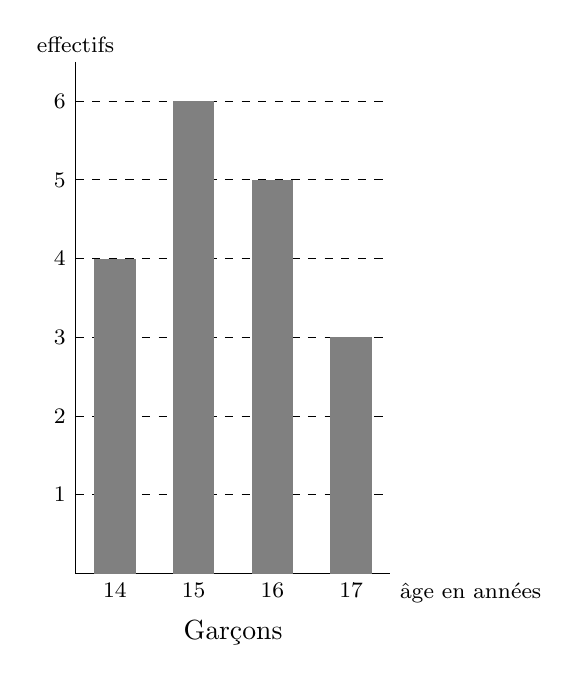
\begin{tikzpicture}
            \foreach \x in {1,2,3,4,5,6} \draw[dashed] (0,\x) -- (4,\x);
            \foreach \x in {1,2,3,4,5,6} \draw (0,\x) node[left] {\footnotesize $\x$};
            \draw[line width = 0.2pt] (0,6.5) node[above] {\footnotesize effectifs} -- (0,0) -- (4,0) node[below right] {\footnotesize âge en années};
            \draw[line width = 15pt,color=gray] (0.5,0) -- (0.5,4);
            \draw[line width = 15pt,color=gray] (1.5,0) -- (1.5,6);
            \draw[line width = 15pt,color=gray] (2.5,0) -- (2.5,5);
            \draw[line width = 15pt,color=gray] (3.5,0) -- (3.5,3);
            \foreach \x in {14,15,16,17} \draw (\x-13.5,0) node[below] {\footnotesize $\x$};
            \draw (2,-0.75) node {\bsc{Garçons}};
        \end{tikzpicture}
        \hspace*{2cm}
        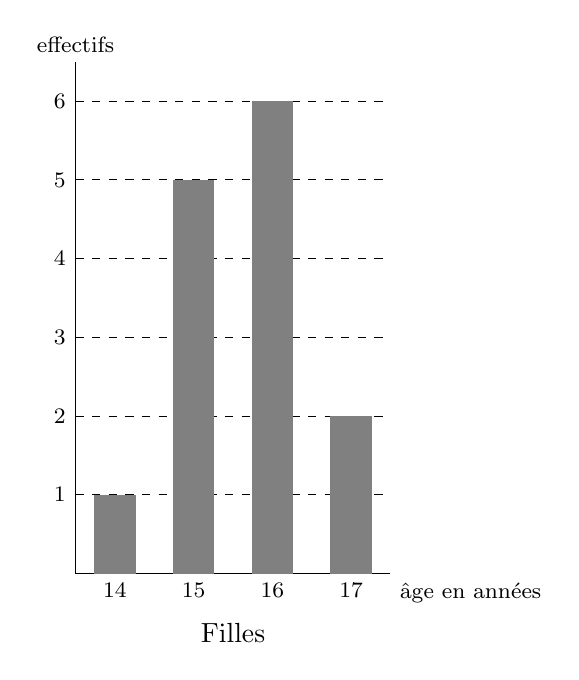
\begin{tikzpicture}
            \foreach \x in {1,2,3,4,5,6} \draw[dashed] (0,\x) -- (4,\x);
            \foreach \x in {1,2,3,4,5,6} \draw (0,\x) node[left] {\footnotesize $\x$};
            \draw[line width = 0.2pt] (0,6.5) node[above] {\footnotesize effectifs} -- (0,0) -- (4,0) node[below right] {\footnotesize âge en années};
            \draw[line width = 15pt,color=gray] (0.5,0) -- (0.5,1);
            \draw[line width = 15pt,color=gray] (1.5,0) -- (1.5,5);
            \draw[line width = 15pt,color=gray] (2.5,0) -- (2.5,6);
            \draw[line width = 15pt,color=gray] (3.5,0) -- (3.5,2);
            \foreach \x in {14,15,16,17} \draw (\x-13.5,0) node[below] {\footnotesize $\x$};
            \draw (2,-0.75) node {\bsc{Filles}};
        \end{tikzpicture}
    \end{center}
    
    \begin{enumerate}
        \item Combien y a t-il de garçons dans la classe ? Justifier en écrivant le calcul effectué.
        \item Combien y a t-il de filles dans la classe ? Justifier en écrivant le calcul effectué.
        \item En utilisant la fonction \texttt{stats} de la calculatrice, déterminer \textbf{pour chaque série} :
        \begin{enumerate}
            \item l'âge moyen ;
            \item l'écart type ;
            \item l'intervalle interquartile.
        \end{enumerate}
        \item \textbf{Interpréter} l'intervalle interquartile des \textbf{filles}.
        \item En explicitant la formule, calculer l'âge moyen de l'ensemble des élèves de la classe.
    \end{enumerate}
\end{exoc}

\vfill

\begin{center}
    \textbf{Tourner la page pour l'exercice 2 !}
\end{center}

\vfill\clearpage

\begin{exoc}{13 points}
    Une machine est programmée pour fabriquer une pièce dont le diamètre doit être de $5~mm$. Pour cela, l'opérateur règle la machine sur cette valeur. On observe toutefois des variations dans les diamètres des pièces fabriquées, ceci est inévitable mais il faut toutefois rester dans des limites acceptables.\par
    Un échantillon de 40 pièces est prélevé en vue de contrôler la machine. Les résultats sont dans le tableau suivant :
    
    \begin{center}
        \begin{tabular}{|>{\bfseries\centering} m{3cm}|*{10}{>{\centering\arraybackslash}m{0.75cm}|}}
            \hline
                Diamètre des pièces (en $mm$)& $4,5$ & $4,6$ & $4,7$ & $4,8$ & $4,9$ & $5$ & $5,1$ & $5,2$ & $5,3$ & $5,4$ \\
            \hline
                Effectifs & $1$ & $1$ & $4$ & $9$ & $10$ & $5$ & $4$ & $2$ & $3$ & $1$ \\
            \hline
                Fréquence \par (en pourcentage) & & & & & & & & & & \\
            \hline
                Fréquence Cumulée Croissante & & & & & & & & & & \\
            \hline
        \end{tabular}
    \end{center}
    
    \begin{enumerate}
        \item Compléter les deux dernières lignes du tableau directement sur le sujet. Donner les résultats sous forme de pourcentage \textbf{sans arrondir}.
        \item
            \begin{enumerate}
                \item Sur le graphique ci-dessous, tracer le polygone des fréquences cumulées croissantes en respectant les graduations.
                \item En laissant apparaître les traits en pointillés sur le graphique, déterminer graphiquement une valeur approchée d'une médiane, des premiers et troisièmes quartiles.
                \item \textbf{Interpréter} les trois valeurs précédentes.
            \end{enumerate}
        \item En explicitant la formule utilisée, \textbf{calculer} la valeur exacte du diamètre moyen des pièces. On le notera $\overline d$.
        \item En utilisant la fonction \texttt{stats} de la calculatrice, déterminer l'écart-type de cette série. Arrondir le résultat à $10^{-3}$ près. On le notera $\sigma$.
        \item Déterminer les intervalles $I_1 = \intervalleff{\overline d - \sigma}{\overline d + \sigma}$ et $I_2 = \intervalleff{\overline d - 2\sigma}{\overline d + 2\sigma}$.
        \item La production de la machine est jugée satisfaisante si environ $66\%$ des pièces appartiennent à l'intervalle $I_1$ et $95\%$ des pièces appartiennent à l'intervalle $I_2$.\par
        La production de la machine est-elle correcte ? Justifier précisément.
    \end{enumerate}\medskip

    \begin{center}
        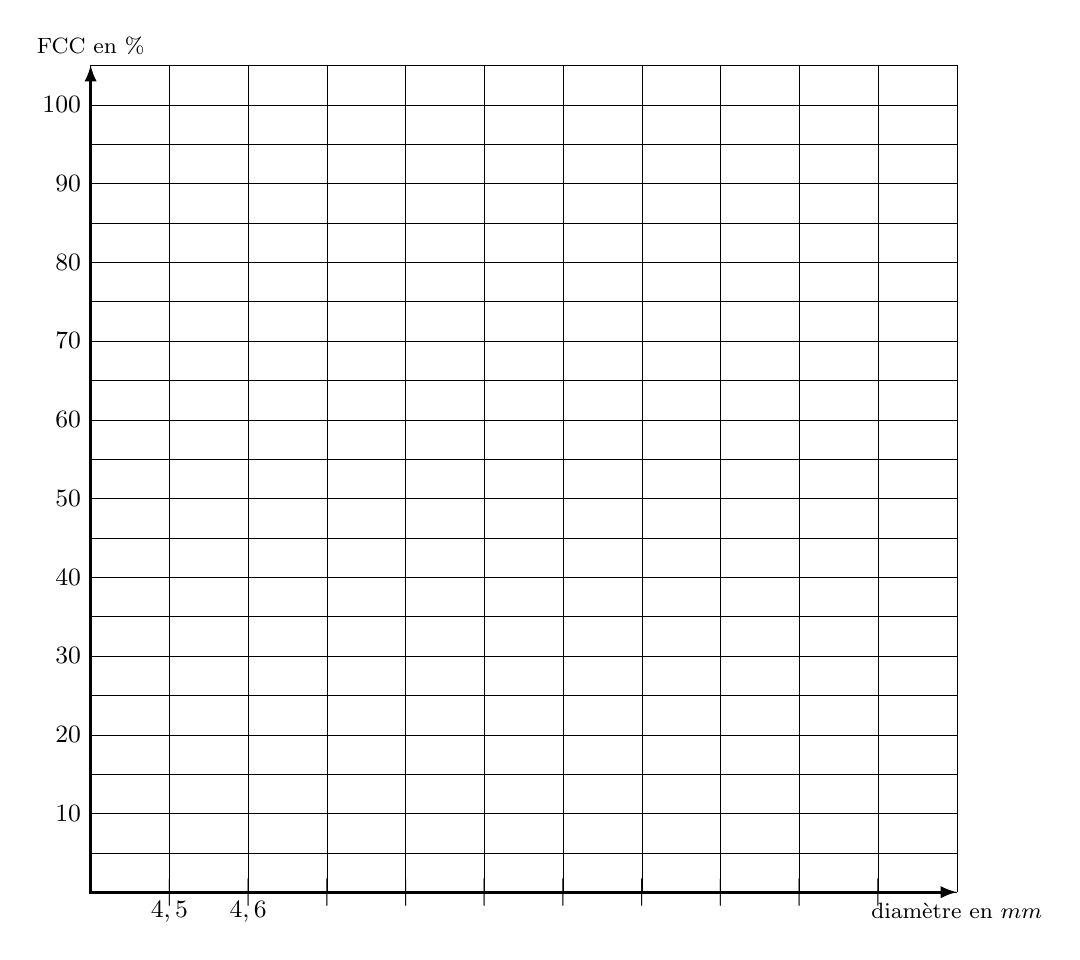
\begin{tikzpicture}[y=0.1cm,>=latex]
            \draw[line width = 0.1pt] (0,0) grid[ystep=5] (11,105);
            \draw[line width = 1pt,<->] (0,105) node[above] {\footnotesize FCC en \%} -- (0,0) -- (11,0) node[below] {\footnotesize diamètre en $mm$};
            \foreach \x in {10,20,...,100} \draw (0,\x) node[left] {\small$\x$};
            \foreach \x in {1,2,...,10} \draw (\x,0) node {$|$};
            \draw (1,0) node[below] {\small $4,5$}; \draw (2,0) node[below] {\small $4,6$};
        \end{tikzpicture}
    \end{center}
\end{exoc}

\clearpage\setcounter{exoc}{0}

%--------------------------------------------------
%       SUJET B
%--------------------------------------------------

\pieddepage{}{B}{}

\begin{center}
\begin{tabularx}{\textwidth}{|c|>\centering X|c|}
	\hline
		1\iere \bsc{e.e.a.c.} &  \bsc{Contrôle de mathématiques} & \textbf{Statistiques} \\
	\hline
		\multicolumn{3}{|c|}{Lundi 30 septembre \np{2013}} \\
	\hline
        \multicolumn{1}{|r}{\bsc{Nom}:} & \multicolumn{2}{l|}{} \\
		\multicolumn{1}{|r}{Prénom:} & \multicolumn{2}{l|}{} \\
	\hline
        \multicolumn{3}{|l|}{\bfseries Note et observations :} \\[1cm]
    \hline
\end{tabularx}\bigskip

{\itshape
La qualité et la précision de la rédaction seront prises en compte dans l'appréciation des copies.\par
Le barème est indicatif.}
\end{center}

\begin{exoc}{7 points}
    On considère les deux séries statistiques ci-dessous représentant les élèves d'une classe en fonction de leur âge.\par
    La série de gauche représente la répartition des garçons et la série de droite celle des filles.\medskip

    \begin{center}
        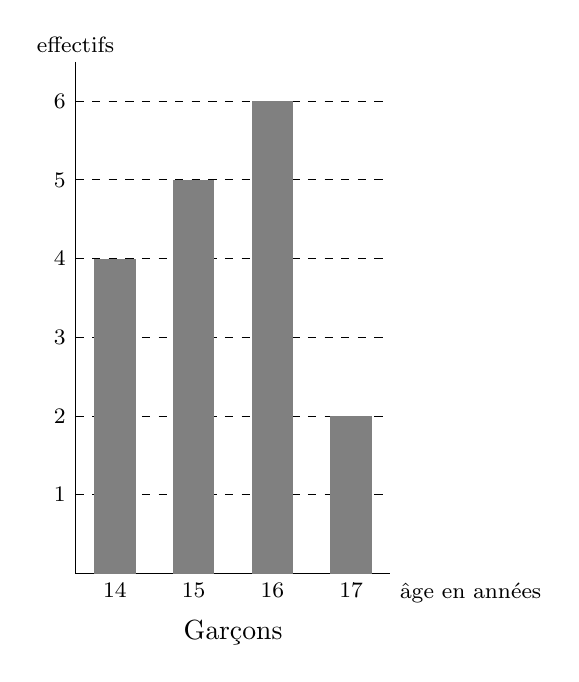
\begin{tikzpicture}
            \foreach \x in {1,2,3,4,5,6} \draw[dashed] (0,\x) -- (4,\x);
            \foreach \x in {1,2,3,4,5,6} \draw (0,\x) node[left] {\footnotesize $\x$};
            \draw[line width = 0.2pt] (0,6.5) node[above] {\footnotesize effectifs} -- (0,0) -- (4,0) node[below right] {\footnotesize âge en années};
            \draw[line width = 15pt,color=gray] (0.5,0) -- (0.5,4);
            \draw[line width = 15pt,color=gray] (1.5,0) -- (1.5,5);
            \draw[line width = 15pt,color=gray] (2.5,0) -- (2.5,6);
            \draw[line width = 15pt,color=gray] (3.5,0) -- (3.5,2);
            \foreach \x in {14,15,16,17} \draw (\x-13.5,0) node[below] {\footnotesize $\x$};
            \draw (2,-0.75) node {\bsc{Garçons}};
        \end{tikzpicture}
        \hspace*{2cm}
        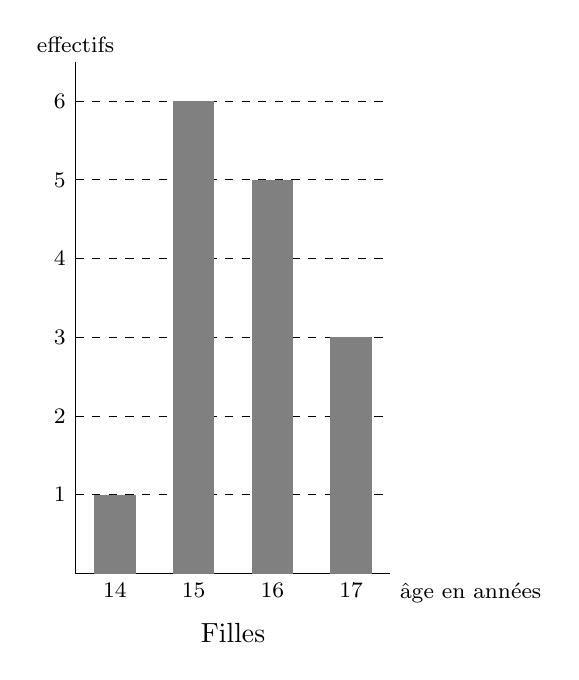
\begin{tikzpicture}
            \foreach \x in {1,2,3,4,5,6} \draw[dashed] (0,\x) -- (4,\x);
            \foreach \x in {1,2,3,4,5,6} \draw (0,\x) node[left] {\footnotesize $\x$};
            \draw[line width = 0.2pt] (0,6.5) node[above] {\footnotesize effectifs} -- (0,0) -- (4,0) node[below right] {\footnotesize âge en années};
            \draw[line width = 15pt,color=gray] (0.5,0) -- (0.5,1);
            \draw[line width = 15pt,color=gray] (1.5,0) -- (1.5,6);
            \draw[line width = 15pt,color=gray] (2.5,0) -- (2.5,5);
            \draw[line width = 15pt,color=gray] (3.5,0) -- (3.5,3);
            \foreach \x in {14,15,16,17} \draw (\x-13.5,0) node[below] {\footnotesize $\x$};
            \draw (2,-0.75) node {\bsc{Filles}};
        \end{tikzpicture}
    \end{center}

    \begin{enumerate}
        \item Combien y a t-il de garçons dans la classe ? Justifier en écrivant le calcul effectué.
        \item Combien y a t-il de filles dans la classe ? Justifier en écrivant le calcul effectué.
        \item En utilisant la fonction \texttt{stats} de la calculatrice, déterminer \textbf{pour chaque série} :
        \begin{enumerate}
            \item l'âge moyen ;
            \item l'écart type ;
            \item l'intervalle interquartile.
        \end{enumerate}
        \item \textbf{Interpréter} l'intervalle interquartile des \textbf{garçons}.
        \item En explicitant la formule, calculer l'âge moyen de l'ensemble des élèves de la classe.
    \end{enumerate}
\end{exoc}

\vfill

\begin{center}
    \textbf{Tourner la page pour l'exercice 2 !}
\end{center}

\vfill\clearpage

\begin{exoc}{13 points}
    Une machine est programmée pour fabriquer une pièce dont le diamètre doit être de $5~mm$. Pour cela, l'opérateur règle la machine sur cette valeur. On observe toutefois des variations dans les diamètres des pièces fabriquées, ceci est inévitable mais il faut toutefois rester dans des limites acceptables.\par
    Un échantillon de 40 pièces est prélevé en vue de contrôler la machine. Les résultats sont dans le tableau suivant :

    \begin{center}
        \begin{tabular}{|>{\bfseries\centering} m{3cm}|*{10}{>{\centering\arraybackslash}m{0.75cm}|}}
            \hline
                Diamètre des pièces (en $mm$)& $4,5$ & $4,6$ & $4,7$ & $4,8$ & $4,9$ & $5$ & $5,1$ & $5,2$ & $5,3$ & $5,4$ \\
            \hline
                Effectifs & $2$ & $1$ & $4$ & $9$ & $10$ & $5$ & $4$ & $2$ & $2$ & $1$ \\
            \hline
                Fréquence \par (en pourcentage) & & & & & & & & & & \\
            \hline
                Fréquence Cumulée Croissante & & & & & & & & & & \\
            \hline
        \end{tabular}
    \end{center}

    \begin{enumerate}
        \item Compléter les deux dernières lignes du tableau directement sur le sujet. Donner les résultats sous forme de pourcentage \textbf{sans arrondir}.
        \item
            \begin{enumerate}
                \item Sur le graphique ci-dessous, tracer le polygone des fréquences cumulées croissantes en respectant les graduations.
                \item En laissant apparaître les traits en pointillés sur le graphique, déterminer graphiquement une valeur approchée d'une médiane, des premiers et troisièmes quartiles.
                \item \textbf{Interpréter} les trois valeurs précédentes.
            \end{enumerate}
        \item En explicitant la formule utilisée, \textbf{calculer} la valeur exacte du diamètre moyen des pièces. On le notera $\overline d$.
        \item En utilisant la fonction \texttt{stats} de la calculatrice, déterminer l'écart-type de cette série. Arrondir le résultat à $10^{-3}$ près. On le notera $\sigma$.
        \item Déterminer les intervalles $I_1 = \intervalleff{\overline d - \sigma}{\overline d + \sigma}$ et $I_2 = \intervalleff{\overline d - 2\sigma}{\overline d + 2\sigma}$.
        \item La production de la machine est jugée satisfaisante si environ $66\%$ des pièces appartiennent à l'intervalle $I_1$ et $95\%$ des pièces appartiennent à l'intervalle $I_2$.\par
        La production de la machine est-elle correcte ? Justifier précisément.
    \end{enumerate}\medskip

    \begin{center}
        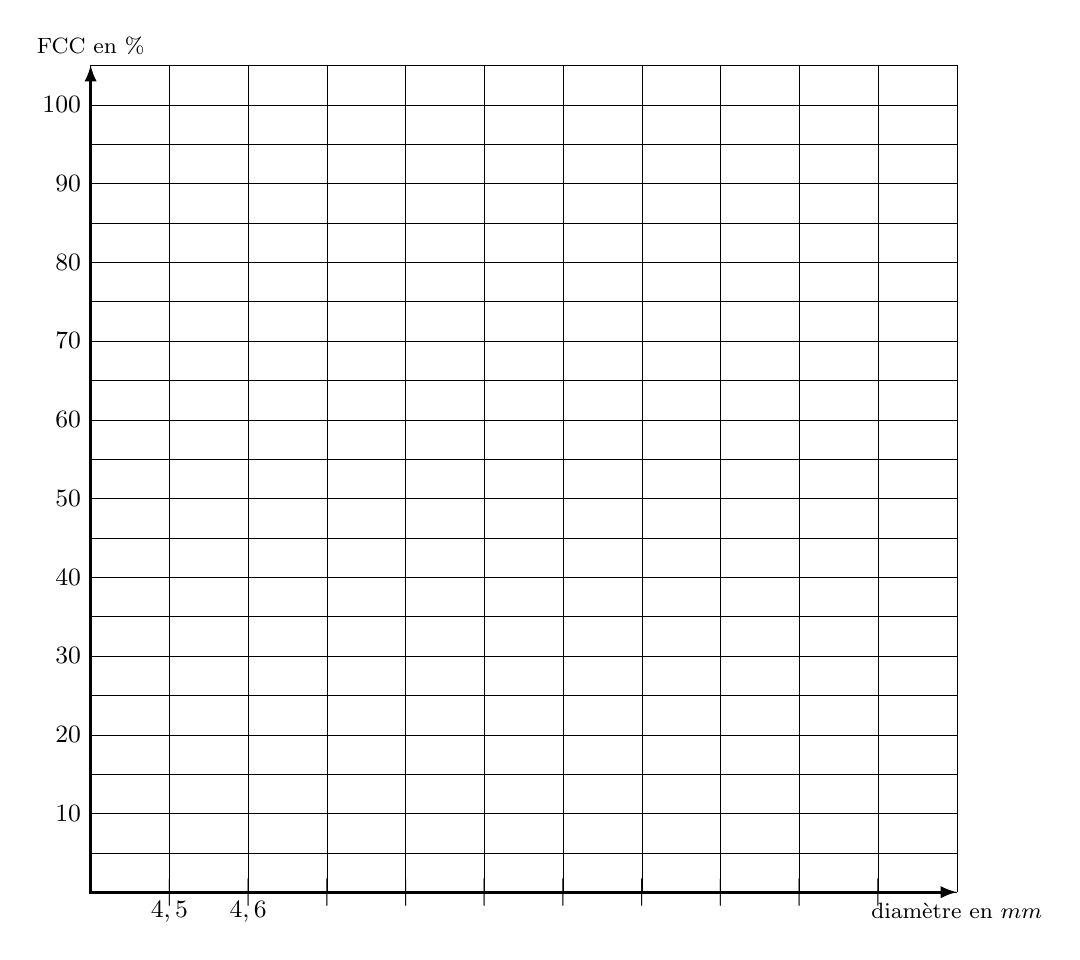
\begin{tikzpicture}[y=0.1cm,>=latex]
            \draw[line width = 0.1pt] (0,0) grid[ystep=5] (11,105);
            \draw[line width = 1pt,<->] (0,105) node[above] {\footnotesize FCC en \%} -- (0,0) -- (11,0) node[below] {\footnotesize diamètre en $mm$};
            \foreach \x in {10,20,...,100} \draw (0,\x) node[left] {\small$\x$};
            \foreach \x in {1,2,...,10} \draw (\x,0) node {$|$};
            \draw (1,0) node[below] {\small $4,5$}; \draw (2,0) node[below] {\small $4,6$};
        \end{tikzpicture}
    \end{center}
\end{exoc}


\end{document} 